%!TEX root = ../thesis.tex
%Adding the above line, with the name of your base .tex file (in this case "thesis.tex") will allow you to compile the whole thesis even when working inside one of the chapter tex files


\chapter{Introduction to Radio Interferometry} \label{chap:2}

The poor spatial resolution provided by a single dish radio antenna can cause difficulties in obtaining accurate flux density measurements of radio astronomical sources, especially at long wavelengths. A single dish radio antenna is unable to distinguish against background radio emitters located in the primary beam, and therefore the observed flux density can contain emission from unrelated sources. This limitation can be overcome through interferometry. An interferometer acts as a spatial filter, and can discriminate against smooth backgrounds, while its higher resolution allows separation of the target from nearby confusing sources. This chapter describes the basic elements of a radio interferometer, what happens to the radio signal before it is sent for correlation, introduces the general concept of interferometry, and  explains the process of synthesis imaging.

\section{Radio Antenna Fundamentals}\label{sec:2.1}

The quality and properties of the final radio image produced from a synthesis array are partially dependent on the properties of the individual antennas in the array. The most important such properties are discussed in the following sections and include aperture size, aperture efficiency, pointing accuracy and sidelobe level. We define the radio antenna as the piece of equipment which converts the electromagnetic waves emitted from the observed source into an electric current ready to be input into to the first low noise amplifier where the signal is at the radio/sky frequency, $\nu _{\rm{RF}}$. What happens to the signal after this will be discussed in Section \ref{sec:2.2}.

\subsection{Properties of a Radio Antenna}\label{subsec:2.1.1}

The power gain of a transmitting antenna is a measure of the antenna's capability of converting power into radio waves in a specific direction. In radio astronomy, the receiving counterpart of transmitting power gain is the effective collecting area of an antenna, $A$($\nu$,$\theta$,$\phi$), where $\nu$ is frequency and $\theta$ and $\phi$ are direction coordinates. An ideal radio antenna would collect all incident radiation from a distant point source and convert it to electrical power. The total spectral power $P_{\nu}$ collected by it would then be a product of its geometric area and the incident spectral power per area, or flux density $F_{\nu}$. By analogy then, the effective area of a real radio antenna is defined
\begin{equation}
A(\nu,\theta,\phi)= \frac{P_{\nu}}{F_{\nu}}=\frac{P}{I(\nu,\theta,\phi)\Delta \nu \Delta \Omega}
\end{equation}
where $I$($\nu$,$\theta$,$\phi$) is the source brightness in units W m$^{-2}$ Hz$^{-1}$ sr$^{-1}$ that the antenna is pointing at and $P$ is the power (in Watts) received by the antenna in bandwidth $\Delta \nu$ from element $\Delta\Omega$ of solid angle. The normalized antenna reception pattern $\mathcal{A}$, often referred to as the power pattern due to the duality between receiving and transmitting, is defined as 
\begin{equation}
\mathcal{A}(\nu,\theta,\phi)= \frac{A(\nu,\theta,\phi)}{A_{0}}
\end{equation}
where $A_0$ (m$^2$) is often referred to as the effective area of the antenna and is the response at the center of the main lobe of $A$($\nu$,$\theta$,$\phi$) [i.e., A($\nu$,0,0)]. Then the beam solid angle, $\Omega _{A}$, of the primary beam is 
\begin{equation}
\Omega _{A} = \int \!\!\! \int _{\rm{all\ sky}} \mathcal{A}(\theta,\phi) d \Omega
\end{equation}
and is a measure of the field of view of the antenna. 

In the case of an isotropic antenna [i.e., $\mathcal{A}(\nu,\theta,\phi)=1$], it can be shown that the product of the effective area and the primary beam solid angle is equal to the square of the wavelength \citep{kraus_1986}
\begin{equation}\label{eq:kraus}
A_{0}\Omega _{A} = \lambda ^2.
\end{equation}
$\Omega _{\rm{A}}$ has its maximum possible value of $4\pi$ if $\mathcal{A}$ is everywhere equal to 1. This means that the primary antenna can see the whole sky with equal sensitivity. Even though a large field of view is usually desirable in radio astronomy, Equation \ref{eq:kraus} ensures that for any given wavelength, when $\Omega _{A}$ is a maximum, the power received is a minimum and therefore the sensitivity is also at a minimum. To improve sensitivity, one could increase the collecting area of the antenna, but Equation \ref{eq:kraus} then ensures that the field of view must decrease. Thus, when deciding on the primary antenna size in a synthesis array, there is always a trade-off between field of view and sensitivity. 

In reality, an antenna cannot radiate isotropically and will radiate preferentially in one or more directions. A Fourier transform relationship exists between the complex voltage distribution of the field, $f(u,v)$, in the aperture of the antenna and the complex far-field voltage radiation pattern, $F(l,m)$, of the antenna \citep{kraus_1986}
\begin{equation}
F(l,m)=\int\!\!\! \int _{\rm{aperture}} f(u,v)e^{2\pi i(ul+vm)}dudv
\end{equation}
and
\begin{equation}\label{eq:illum1}
f(u,v)=\int ^{\infty} _{\infty}\int ^{\infty} _{\infty} F(l,m)e^{-2\pi i(ul+vm)}dldm
\end{equation}
where
\begin{equation}\label{eq:illum2}
u=\rm{sin}\theta \rm{cos}\phi \ \  \rm{and} \ \ \mathit{v}=\rm{sin}\theta \rm{sin}\phi
\end{equation}

\begin{figure}[H]
\centering 
\mbox{
          \includegraphics[trim=60pt 10pt 80pt 30pt,clip,width=7.0cm]{/home/eamon/thesis/figures/antenna_beam/fig2a.ps}
          \includegraphics[trim=60pt 10pt 80pt 30pt,clip,width=7.0cm]{/home/eamon/thesis/figures/antenna_beam/fig2b.ps}
          }
\mbox{
          \includegraphics[angle=90,trim= 10pt 80pt 30pt 60pt,clip,width=8.0cm]{/home/eamon/thesis/figures/antenna_beam/fig2c.ps}
          }
\caption[Radiation and power pattern of a uniformly illuminated antenna.]{\textit{Top Left:} A uniformly illuminated 1-D aperture $f(u)$. \textit{Top Right:} The Fourier transform of $f(u)$ gives the antenna radiation pattern in the far-field, $F(l)$. \textit{Bottom:} The power pattern of the antenna is given by $\mathcal{A}=|F(l)|^2$.}
\label{fig2.1}
\end{figure}

are the antenna coordinates and $l$ and $m$ are their Fourier counterparts. The from of $f(u,v)$ is determined by the manner in which the antenna feed illuminates the aperture. Therefore Equations \ref{eq:illum1} and \ref{eq:illum2} tell us that the radiation pattern in the far-field of a two-dimensional aperture is the two-dimensional Fourier transform of the aperture field illumination. For a uniformly illuminated 1-D aperture shown in Figure \ref{fig2.1}, the radiation pattern in the far-field is the \textit{sinc} function. The radiation pattern in the far-field, $F(l,m)$, of such an antenna is related to the antenna power pattern by $\mathcal{A}=|F(l,m)|^2$. This power pattern is known as the Airy pattern if the antenna is uniformly illuminated and is also shown in Figure \ref{fig2.1}. The central peak of this power pattern is called the main beam while the smaller secondary peaks are called sidelobes. The antenna is maximally sensitive to radiation from the direction of the peak of the beam, but is also slightly sensitive to radiation in the direction of the side lobes. The half-power beamwidth (HPBW) of the main beam $\theta_{\rm{HPBW}}$ is a term commonly used in the literature to describe the field of view of an antenna/interferometer and satisfies 
\begin{equation}
\theta_{\rm{HPBW}} \propto \frac{\lambda}{D}
\end{equation}
where $D$ is the diameter of the antenna. The constant of proportionality varies slightly with the illumination taper and can be shown to be equal to $\sim 0.89$ for a uniformly illuminated 1-D aperture and $\sim 1.2$ for most single dish radio antennas. When the sky is scanned with a single dish antenna, then this HPBW is the resolution of the resulting map. 
\subsection{Antenna Structural Design}\label{subsec:2.1.2}
The design of the primary antenna element of an interferometric array will depend on the wavelength range to be observed. In general, dipoles are used for wavelengths longer than $\sim 1$ m, while reflector antennas are typically used at shorter wavelengths. The reason why the more simple and less expensive dipoles are not used at all wavelengths is given by Equation \ref{eq:kraus}. For an isotropic antenna, this equation tells us that the effective area is just
\begin{equation}
A_{0} = \frac{\lambda ^2}{4\pi}.
\end{equation}
Therefore, at short wavelengths a non-directional antenna such as a dipole, will have a small effective collecting area, giving it poor sensitivity for reception. Thus, dipoles can be used at long wavelengths as they have sufficient collecting area, but cannot be used at shorter wavelengths as an impractical amount would be needed to produce useful collecting areas. Since the interferometric arrays used in this thesis use reflector antennas, the rest of this section will focus on them.\\
\\
\textit{Choice of Antenna Mount.} Nearly all interferometric arrays consist of antennas which have altitude over azimuth (alt-azimuth) mounts. These antennas lie on a horizontal azimuth track on which the antenna can turn in azimuth, and on a horizontal elevation axle about which the antenna can change in zenith angle. The main advantage of such a design is simplicity and thus lower cost. Gravity always acts on the reflector in the same plan thus reducing the problem of keeping the reflector profile accurate during the duration an observation. However, sources close to the zenith can usually not be observed due to the high rate of azimuth rotation required. Also, the beam rotates with respect to the source for long duration observations which can affect the dynamic range of total intensity images of very large sources. The other type of mount occasionally used is the equatorial mount. Its polar axis is aligned parallel to the axis of rotation of the Earth and therefore only needs to rotate about the declination axis to observe a source. Its beam also doesn't have the beam rotation problem encountered by the alt-azimuth design and can track sources close to the zenith. Its major disadvantage and the reason for its scarce usage is the complexity of its design and resulting increased cost. \\
\\
\textit{Choice of Antenna Optics.} In Figure \ref{fig2.2} we show the main optical systems which can be used to feed a large radio reflector. The prime focus system (e.g. used in the Giant Meter Radio Telescope) has the advantage that it can be used at long wavelengths where the use of secondary focus feeds (i.e., sub-reflectors) become impractical. However, access to and space for the feeds and receivers are limited, and sensitivity can be lost due to spillover noise from the ground. The other designs have the advantage of easier access to the feeds and receivers and less spillover noise from the ground. The off-axis Cassegrain (e.g. used in the Very Large Array) also has the advantage of increased frequency capability as many feeds can be located in a circle around the center of the reflector and a slight rotation of the sub-reflector is all that is required to change observing frequency. The receivers and feeds in the Naysmith geometry (e.g used in the Combined Array for Research in Millimeter wave Astronomy) are located externally to the antenna structure. Finally, the offset Cassegrain (e.g. used in the Green Bank Telescope) has no blockage and will have a circularly symmetric beam with low sidelobes although the increase complexity of its structure leads to increased costs. 

\begin{figure}[hbt!]
\centering 
          \includegraphics[trim=10pt 40pt 60pt 50pt,clip,width=10.0cm,angle=-90]{/home/eamon/thesis/figures/fig2d.ps}
\caption[Common optical systems used for radio antennas.]{Common optical systems used for radio antennas. (\textit{a}) Prime focus, (\textit{b}) Naysmith, (\textit{c}) Off-axis Cassegrain, (\textit{d}) Offset Cassegrain [Figure adapted from \cite{taylor_1999}].}
\label{fig2.2}
\end{figure}

\subsection{Antenna Performance Parameters}\label{subsec:2.1.3}
\textit{Aperture Efficiency.} The geometric collecting area of a parabolic antenna $A_{\rm{geo}}$ ($=\pi D^2/4$) is related to the effective area (i.e., the collecting area when pointing directly at a source) via the dimensionless quantity $\eta$ ($\eta < 1$) known as the aperture efficiency where
\begin{equation}
\eta = \frac{A_0}{A_{\rm{geo}}}.
\end{equation}
The aperture efficiency directly impacts on the sensitivity of the interferometric array and can be defined as the product of a number of different efficiency loss factors, 
\begin{equation}
\eta = \eta _{\rm{sf}}\eta _{\rm{bl}}\eta _{\rm{s}}\eta _{\rm{t}}\eta _{\rm{misc}}.
\end{equation}
The surface efficiency $\eta _{\rm{sf}}$ accounts for the aperture efficiency loss as a result of reflector profile inaccuracies. Such inaccuracies result in the electric field from various parts of the aperture not adding together in phase at the feed leading to a decrease in power. The aperture blockage efficiency $\eta _{\rm{bl}}$ accounts for the fact that the sub-reflector (or feed) and its support structure result in a reduction in the incident radiation on the antenna. The feed spillover efficiency $\eta _{\rm{bl}}$ is best understood if the antenna is considered in transmission rather than in reception mode, and  is defined as the fraction of power radiated by the feed that is intercepted by the reflector for a prime focus system, or by the sub-reflector for a Cassigrain system. The illumination taper efficiency $\eta _{\rm{t}}$ accounts for the fact that the feed pattern does not illuminate the primary reflector uniformly but illuminates the outer part of the reflector at a lower level than the inner part. Finally, the miscellaneous efficiency losses such as reflector diffraction and feed position phase errors are accounted for in $\eta _{\rm{misc}}$. As an example, the total aperture efficiency of the VLA antennas can vary between 0.65 and 0.2 at 6 and 0.7 cm, respectively.
\\
\\
\textit{Pointing Accuracy.}
The main lobe of an antenna's power pattern will usually not point exactly in the desired direction due to gravity deformations, wind pressure deformations, and mechanical inaccuracy. The angular offset, $\Delta \theta$, between the actual and desired pointing direction is called the pointing error. Usually, the desirable pointing error of  an antenna at the highest operational frequency is $\Delta \theta < \theta _{\rm{HPBW}}/20$ \citep{taylor_1999}. With this specification reached, an antenna pointing at a compact source will suffer negligible intensity variations as $\mathcal{A}(\theta _{\rm{HPBW}}/20) > 0.99$. However, this pointing error of only $\theta _{\rm{HPBW}}/20$ will still have a substantial effect on the accuracy of the outer image. For example, a source located at the half power point will suffer a substantial fractional intensity variation of $2\mathcal{A}(\theta _{\rm{HPBW}}/2+\theta _{\rm{HPBW}}/20) \simeq 0.86$. The blind pointing of a VLA antenna is only about 10$^{\prime\prime}$ and can be much worst in daytime, occasionally exceeding 1$^{\prime}$. This means that at Q-band (45 GHz; 0.7 cm), which is the highest observing frequency on the VLA, the pointing error is only at best $\theta _{\rm{HPBW}}/6$, and at worst $>\theta _{\rm{HPBW}}$, meaning that the target may lie outside of the primary beam. To overcome this problem of large antenna pointing errors at high frequencies with the VLA, a technique known as referenced pointing is implemented. This technique will be discussed further in Chapter 3. 

\section{Receiving System for an Interferometer}\label{sec:2.2}

A radiometer (a radio receiver) is a device  used to measure the  timed-averaged power of the noise coming from a radio telescope within a  well-defined radio frequency (RF) range, $\nu _{\rm{RF}}-\Delta \nu _{\rm{RF}}/2 \rightarrow \nu _{\rm{RF}}+\Delta \nu _{\rm{RF}}/2$, where $\Delta \nu _{\rm{RF}}$ is the bandwidth of the receiver and $\Delta \nu _{\rm{RF}}< \nu _{\rm{RF}}$. 
The simplest radiometer carries out the following tasks:
\begin{enumerate}
\item Filters the broadband noise coming from the antenna via a bandpass filter.
\item Multiplies the filtered voltage by itself (i.e., its output voltage is proportional to its input power).
\item Smooths out the rapidly fluctuating output of the detected voltage via a a signal averager or integrator.
\item Measures the smoothed voltage.
\end{enumerate}
In practice, radiometers are never as simple as those described above and nearly all practical radiometers are \textit{superheterodyne} receivers which incorporate a number of additional steps to produce an output voltage.

The RF front end is the term used to describe all the circuitry between  the feed horn and the lower intermediate frequency (IF) stage. The first task of the front end is to amplify the received signal. The radio signals we want to measure are generally very weak and therefore need to be initially amplified by many orders of magnitude so they are above the noise level in succeeding stages. However, the front end electronic components produce random electrical noise which will also get amplified by this large amount. Therefore the role of the pre-amplifier is to amplify the incoming signal from the antenna while adding as little noise as possible. For this reason, the pre-amplifier is often called a low noise amplifier (LNA) and are often cooled to very low temperatures to minimize the amount of noise contributed by the components.

\begin{figure}[hbt!]
\centering 
          \includegraphics[trim=0pt 350pt 0pt 320pt,clip,width=15.0cm]{/home/eamon/thesis/figures/front_end.ps}
\caption[Block diagram of a superheterodyne receiver.]{\textit{Left:} Block diagram of a simple superheterodyne receiver. The amplified RF signal is mixed with a signal from a local oscillator to convert the signal to the more manageable intermediate frequency. \textit{Right:} For interferometry, a phase lock loop is used to ensure all antennas are locked to the same frequency.}
\label{fig2.3}
\end{figure}

The amplified RF signal is then sent through a mixer which multiplies the RF signal by a sine wave of frequency $\nu _{\rm{LO}}$ which is generated by a local oscillator (LO), as shown in Figure \ref{fig2.3}. The effect of this is that RF signal is changed to a lower frequency which can be easier handled by the IF amplifier and  improves frequency selectivity. Mathematically, the mixer does the following
\begin{equation}
2\rm{sin}(2\pi \nu _{\rm{LO}}\mathit{t})\times \rm{sin}(2\pi \nu _{\rm{RF}}\mathit{t}) = \rm{cos}[2\pi (\nu _{\rm{LO}}-\nu _{\rm{RF}})\mathit{t}]-\rm{cos}[2\pi (\nu _{\rm{LO}}+\nu _{\rm{RF}})\mathit{t}],
\end{equation}
and produces two additional outputs, one at the input signal frequency minus the local oscillator frequency, and one at the sum of these frequencies. The lower of the two outputs called the intermediate frequency (IF) is taken by passing the mixer output through a filter in the IF amplifier. In interferometry, where the signals from two antennas are correlated, it is crucial that the receivers from both antennas are operating at the same frequency to control the phase difference between them. This is achieved by using a phase lock system, whose block diagram is laid out in Figure \ref{fig2.3}. In this system another mixer compares the LO to a reference frequency, which is the same for all antennas. Any existing phase error results in an error signal that is sent back to the oscillator so that its frequency can be adjusted to maintain exact frequency tuning. After this, the IF can finally be sent to the radiometer and recorded.

\section{Fundamentals of Radio Interferometry}\label{sec:3}
The angular resolution $\Delta \theta$ of a radio antenna is the minimum angular separation which two point sources can have in order to be recognized as separate objects. The \textit{Rayleigh criterion} is the generally accepted criterion for defining the angular resolution of a filled circular aperture of diameter $D$, at the observational wavelength $\lambda$ and is given as
\begin{equation}
\Delta \theta=1.22\frac{\lambda}{D} \ \ \rm{rad}.
\label{eq:rayleigh}
\end{equation}
The Rayleigh criterion states that two objects are resolved when the first null of the diffraction pattern of one object coincides with the maximum of the diffraction pattern of the other. An immediate consequence of Equation \ref{eq:rayleigh} is that at large wavelengths, the angular resolution becomes large unless the diameter of the aperture can be increased substantially. In order to achieve modest angular resolution at radio wavelengths with a single radio antenna then, the diameter becomes impractically large. For example, in order to achieve an angular resolution of 1$^{\prime \prime}$ at 6 cm a 12 km aperture would be required. Radio interferometry is a technique used in radio astronomy to overcome this problem of poor angular resolution at long wavelengths. 

\subsection{Young's Slits}\label{subsec:4}
The basic principles of interferometry can be understood through Young's double-slit experiment. If coherent radiation emitted from a distant point source propagates through two slits, an illumination pattern composed of bright and dark fringes is observed. The phenomenon is a result of the constructive and destructive interference between the secondary waves produced by the slits. The fringe separation is $\lambda /B$, where $B$ is the projected separation of the slits and is called the baseline. The fringe contrast which is historically known as the fringe visibility, $V$, can be written as
\begin{equation}
|V| = \frac{I_{\rm{max}}-I_{\rm{min}}}{I_{\rm{max}} + I_{\rm{min}}}
\end{equation}
where $I_{\rm{max}}$ and $I_{\rm{min}}$ are the maximum and minimum intensity of the fringes, respectively. In other words, the fringe visibility is the fringe amplitude normalized by the sum of the maximum and minimum intensity. 

\begin{figure}[hbt!]
\centering 
          \includegraphics[trim=0pt 0pt 0pt 0pt,clip,width=12.0cm]{/home/eamon/thesis/figures/youngs.ps}
\caption[Fringe pattern produced by Young's slits under various situations.]{The resulting fringe pattern produced by Young's slits under various conditions. The source is shown on the left of the slits in each panel, while the separate fringe patterns (colors) along with the added fringe pattern (black) is shown on the right of the slits. (\textit{a}) Point source at infinity, (Visibility = 1). Fringes are separated by an angular distance of $\lambda /B$. (\textit{b}) An increase in source size results in a drop in visibility. (\textit{c}) When the source size is equal to $\lambda /B$, the visibility is zero. (\textit{d}) If the source size remains the same as in (c) and the slit spacing is reduced, then the fringes re-appear. Figure adapted from \cite{jackson_2008}.}
\label{fig2.4}
\end{figure}

In the simple case shown in Figure \ref{fig2.4}a, the angular size of the source is  $\ll \lambda/B$ and the fringe visibility is 1. In interferometry, this equates to the situation in which the source size is smaller than the synthesized beam and only an upper limit of the source size can be obtained (i.e., the source is unresolved). In Figure \ref{fig2.4}b, the angular size of the source is now larger and can be thought of as a sequence of point sources each emitting radiation which is uncorrelated with emission from the others. An angular shift of $\phi$, called phase, in the sources position results in a shift in the corresponding fringe pattern by the same angle the other way. The total interference intensity pattern is then just the sum of these individual patterns and the visibility is reduced. When the extension of the source equals $\lambda/B$, the fringes disappear and give a constant illumination pattern. In this case the fringe visibility is zero and the source is completely resolved as shown in Figure \ref{fig2.4}c. Finally, if the source size is the same as that in Figure \ref{fig2.4}c but the slit separation is reduced, then the fringe separation $\lambda/B$ will again increase as shown in Figure \ref{fig2.4}d. This is because the source now produces much less displacement of the fringe patterns as a fraction of the fringe separation. In interferometry, this result means that extended sources can only be probed with short baselines. 

Visibility and phase are often expressed together as the complex visibility $V=|V|e^{i\phi}$, which completely defines a pattern of interference fringes. Young's double-slit experiment demonstrates a fundamental property of interferometry, namely that the contrast of fringes is a function of the geometry of the source. The results of the experiment are summarized in Figure \ref{fig2.5}. The top row shows that a large source (i.e., one whose intensity distribution extends out to a large angle on the sky) has a fringe visibility pattern which falls off quickly as projected baseline length increases. The bottom row shows that for compact sources the fringe visibility remains high out to large baselines. In the following section we will show that the relationship between the sky brightness distribution $I(\theta)$ and the visibility $V(B)$ is a Fourier transform.

\begin{figure}[hbt!]
\centering 
          \includegraphics[trim=0pt 270pt 0pt 250pt,clip,width=12.0cm]{/home/eamon/thesis/figures/visibility.ps}
\caption[Visibilities for various source sizes.]{\textit{Left column:} Intensity distribution as a function of sky angle for an extended source (top) and for a more compact source (bottom). \textit{Right column:} The corresponding fringe visibility as a function of slit separation or baseline. Figure adapted from \cite{jackson_2008}.}
\label{fig2.5}
\end{figure}

\subsection{The Two-element Interferometer}\label{subsec:5}
Interferometers with $N$ antennas can be treated as $N(N-1)/2$ independent interferometer pairs so it is worthwhile studying the simplest case of the two-element interferometer. A simplified block diagram of the components of such an interferometer is shown in Figure \ref{fig2.6}. The figure shows two identical antennas separated by a baseline vector \textbf{b} pointing towards a distant radio source in a direction indicated by the unit vector \textbf{s}. The plane waves from the distant radio source reach antenna 1 at a time $\tau _g$ later than they reach antenna 2. $\tau _g$ is called the geometric delay and is given by
\begin{equation}
\tau _{g}=\frac{\textbf{b}.\textbf{s}}{c}=\frac{b\rm{cos}\theta}{c}
\end{equation}
where $c$ is the speed of light. If we assume that the interferometer only responds to a very narrow band centered on frequency $\nu=\omega /2\pi$, then the output voltages of antennas 1 and 2 at time $t$ can be written as 
\begin{equation}
V_1(t)=V\rm{cos}[\omega(\mathit{t}-\tau _g)] \ \ \ \rm{and} \ \ \ \mathit{V_{\rm{2}}(t)=V\rm{cos}(\omega \mathit{t})}.
\end{equation}
The signals are then passed through a correlator which first multiplies these voltages to give
\begin{equation}
V_1(t) V_2(t)=\frac{V^2}{2}[\rm{cos(2\omega t -\omega \tau _g)+\rm{cos}(\omega \tau _g)}]
\end{equation}
and then averages them over a time interval $\Delta t$ which is long enough such that $\Delta t >> (2\omega)^{-1}$ to give the final output $R$:
\begin{equation}
R=\langle V_1(t)V_2(t)\rangle = \frac{V^2}{2}[\rm{cos}(\omega \tau _g)].
\end{equation}

\begin{figure}[hbt!]
\centering 
          \includegraphics[trim=20pt 160pt 20pt 160pt,clip,width=12.0cm]{/home/eamon/thesis/figures/2_el.ps}
\caption[Simplified schematic diagram of a two-element interferometer.]{Simplified schematic diagram of a two-element interferometer. The correlator multiplies and averages the voltage outputs $V_1$ and $V_2$ of the two dishes and yields an output amplitude $V^2/2$ which is proportional to the point-source flux density $F_{\nu}$. \textit{Image Credit:} National Radio Astronomy Observatory.}
\label{fig2.6}
\end{figure}

As the Earth rotates, $\tau _g$ varies slowly with time and the resultant oscillations in the correlator output voltage represent the motion of the source. These sinusoidal oscillations are called fringes, and the fringe phase is 
\begin{equation}
\phi = \omega \tau _g = \frac{\omega b\rm{cos} \theta}{c}
\end{equation}
which changes with source direction as follows
\begin{equation}
\frac{d\phi}{d\theta}= \frac{\omega b\rm{sin} \theta}{c}=2\pi\left(\frac{b\rm{sin}\theta}{\lambda}\right).
\end{equation}
The fringe phase completes a full period (i.e., $\Delta \phi=2\pi$) when an angular change $\Delta \theta=(\lambda/b\rm{sin}\theta)$ occurs. This tells us that the fringe phase is an extremely sensitive measure of source position if the projected baseline $b\rm{sin}\theta$ is many wavelengths long and is the reason why interferometers can determine the positions of compact radio sources with exquisite accuracy.

\begin{figure}[hbt!]
\centering 
          \includegraphics[trim=20pt 180pt 20pt 160pt,clip,width=12.0cm]{/home/eamon/thesis/figures/synth_beam.ps}
\caption[The instantaneous point source responses of an interferometer.]{The instantaneous point source responses of an interferometer with two, three and four elements is indicated by the thick curves. The individual responses of the three pairs of two-element interferometers of the three-element interferometer and the six pairs of two-element interferometers of the four-element interferometer are plotted as thin curves. The main beam of the four-element interferometer is nearly Gaussian and has a width of $\sim \lambda /B$. This is known as the instantaneous synthesized beam of the interferometer. \textit{Image Credit:} National Radio Astronomy Observatory.}
\label{fig2.7}
\end{figure}

If the antennas in an interferometric array are isotropic, then the  point-source response of the interferometer would be a sinusoid spanning the entire sky and the interferometer would be only sensitive to one Fourier component of the sky brightness distribution having angular period $\lambda/b\rm{sin}\theta$. The response of a two-element interferometer $R$ with non-isotropic antennas is this sinusoid multiplied by the product of the voltage patterns (i.e., defined as $f(u,v)$ in Section \ref{subsec:2.1.1}) of the individual antennas. If the antennas are identical then this product is the power pattern of the individual antennas called the primary beam. The primary beam is usually a Gaussian that is much wider than the fringe period as $D << b\rm{sin}\theta$. The result is that an interferometer with directive antennas responds to a finite range of angular frequencies centered on $b\rm{sin}\theta /\lambda$. The instantaneous point source response of an interferometer is known as the synthesized beam and is the point source response obtained by averaging the outputs of all antenna pairs. The synthesized beam of an interferometer is an important quantity as it defines the maximum angular resolution of the instrument. The synthesized beams produced by an interferometer with a various number of antennas arranged in 1-D is shown in Figure \ref{fig2.7}. The figure shows that the synthesized beam can be improved by acquiring more Fourier components (i.e., baselines) and rapidly approaches a Gaussian as $N$ increases. However, sidelobes are still significant and a broad negative ``bowl'' exists between the main beam and the first sidelobes due to the absence of short spacings.

\subsection{Complex Visibility}\label{subsec:6}
The interferometer output can be expressed in terms of the radio brightness over the sky, which is sometimes also called specific intensity and has units W m$^{-2}$ Hz$^{-1}$ sr$^{-1}$. If the radio brightness of a spatially incoherent extended source in the direction of unit vector \textbf{s} is $I$(\textbf{s}), then the response of the two-element interferometer with ``cosine'' correlator output near frequency $\nu =\omega/2\pi$ is obtained by treating the extended source as the sum of independent point sources:
\begin{equation}
R_{c}=\int _{\Omega}\mathcal{A}(\textbf{s})I_{\nu}(\textbf{s}) \rm{cos}\left(\frac{2\pi \textbf{b}.\textbf{s}}{\lambda} \right)d\Omega
\end{equation}
where $\mathcal{A}$ is the normalized antenna reception pattern defined in Section \ref{subsec:2.1.1} and we call $\mathcal{A}(\textbf{s})I_{\nu}(\textbf{s})$ the modified brightness distribution. However, the cosine function in the  ``cosine'' correlator output is only sensitive to the even part of the sky brightness distribution, which can be written as the sum of even and odd parts:
\begin{equation}
I(\textbf{s})=I_{\rm{e}}(\textbf{s})+I_{\rm{o}}(\textbf{s}).
\end{equation}
A ``sine'' correlator whose output is odd, is needed to detect the odd part of $I(\textbf{s})$ and this is implemented by inserting a 90$^{\circ}$ phase delay into the signal of one of the antennas to give
\begin{equation}
R_{s}=\int _{\Omega}\mathcal{A}(\textbf{s})I_{\nu}(\textbf{s}) \rm{sin}\left(\frac{2\pi \textbf{b}.\textbf{s}}{\lambda} \right)d\Omega
\end{equation}

It is convenient to write the cosines and sines as complex exponentials using the identity 
\begin{equation}
e^{i\phi} = \rm{cos}(\phi) + \mathit{i}\rm{sin}(\phi)
\end{equation}
and so the combination of ``cosine'' and ``sine'' correlators is called a ``complex'' correlator. The term \textit{visibility} was first introduced by \cite{michelson_1890} to describe the relative amplitudes of the optical fringes that he observed. The visibility is a complex quantity in radio astronomy and has dimensions of spectral power flux density (W m$^{-2}$ Hz$^{-1}$). The complex visibility is the response of a two-element interferometer with a complex correlator to an extended source with brightness distribution $I(\textbf{s})$  and is defined as
\begin{equation}
V\equiv R_{\rm{c}}-iR_{\rm{s}},
\end{equation}
i.e.,
\begin{equation}
V _{\nu} = \int _{\Omega}\mathcal{A}(\textbf{s})I_{\nu}(\textbf{s})\mathit{e}^{-2\pi \mathit{i} \nu \textbf{b}.\textbf{s}/c}d\Omega .
\label{eq:visib}
\end{equation}
\subsection{Coordinate Systems for Imaging}\label{subsec:7}
The baseline vector \textbf{b} has coordinates ($u,v,w$) in three dimensions shown in Figure \ref{fig2.8} where $w$ points in the directions of interest, i.e., towards a direction \textbf{$s_{0}$} that becomes the center of the synthesized image. $u$, $v$ and $w$ are measured in wavelengths (i.e., the components of $\textbf{b}/\lambda$) and have directions towards the East, the North and the phase tracking center, respectively. An arbitrary unit vector \textbf{s} has components ($l,m,n$) called direction cosines, where $n=\rm{cos}\theta=(1-\mathit{l}^2-\mathit{m}^2)^{1/2}$. Using these coordinates the parameters in Equation \ref{eq:visib} become
\begin{equation}
\begin{split}
\frac{\nu \textbf{b}.\textbf{s}}{c}&=ul+vm+wn, \\
d\Omega &= \frac{dl\,dm}{n}=\frac{dl\,dm}{\sqrt{1-l^2-m^2}}.
\end{split}
\end{equation}
Therefore Equation \ref{eq:visib} can be defined in terms of the coordinate system laid out in Figure \ref{fig2.8} as
\begin{equation}\label{eq:3-d_vis}
\begin{split}
&V_{\nu}(u,v,w)=\\
&\int ^{\infty}_{-\infty}\int ^{\infty}_{-\infty} \mathcal{A}_{\nu}(l,m)I_{\nu}(l,m)\mathit{e}^{-2\pi \mathit{i}[ul+vm+w(\sqrt{1-l^2-m^2})] }\frac{dl\,dm}{\sqrt{1-l^2-m^2}}
\end{split}
\end{equation}
which is not a three-dimensional Fourier transform. This equation becomes a two-dimensional Fourier transform if $w=0$ which is a good approximation for small field imaging, i.e., when $|l|$ and $|m|$ are small. In this case Equation \ref{eq:3-d_vis} can be inverted to find the modified sky brightness distribution:
\begin{equation}\label{eq:2dft}
\mathcal{A}_{\nu}(l,m)I_{\nu}(l,m)=\int ^{\infty}_{-\infty}\int ^{\infty}_{-\infty}V_{\nu}(u,v)\mathit{e}^{2\pi \mathit{i}(ul+vm)}du\,dv.
\end{equation}
Therefore Equation \ref{eq:2dft} demonstrates the important Fourier Transform relationship between the sky brightness distribution and the complex visibility (i.e., the interferometer response).

\begin{figure}[hbt!]
\centering 
          \includegraphics[trim=20pt 200pt 20pt 200pt,clip,width=10.0cm]{/home/eamon/thesis/figures/3dvis.ps}
\caption[The ($u,v,w$) interferometric coordinate system.]{The ($u,v,w$) interferometric coordinate system. $l$, $m$, and $n$ are the projections of the unit vector \textbf{s} onto the $u$, $v$, and $w$ axes, respectively.}
\label{fig2.8}
\end{figure}

\section{Synthesis Imaging}\label{sec:4}
A synthesis imaging telescope consists of a number radio antennas fixed on the ground and uses the Earth's rotation to vary the projected baseline coverage to increase the sampling of the $u-v$ plane. In this section we describe how Earth-rotation aperture synthesis is used to convert the complex visibilities outputted from the correlator to a final radio image of the observed sky.
\subsection{Visibility Sampling}\label{subsec:4.1}
An example of how a radio interferometer samples the $u-v$ plane is shown in Figure \ref{fig2.9}. The left panel of this figure shows the overhead view of the VLA in its most extended configuration while the other two panels shows the corresponding $u-v$ coverage for different periods of time. We define $u$ and $v$ as the east-west and north-south components of the projected baseline in wavelengths, respectively. As the Earth rotates, the projected baseline of every two-element pair in the array changes, thus sampling a different part of the $u-v$ plane. The middle panel shows that the total $u-v$ coverage of the VLA for a very short duration track (i.e., a snapshot) results in a `snowflake' like pattern, with more dense coverage in the direction of the arms of the array due to the larger number of baselines. Most radio interferometers have their own unique array configuration layout and thus produce a different `snapshot' $u-v$ coverage to that shown in Figure \ref{fig2.9}. Over many hours, the $u-v$ points trace out portions of ellipses and eventually after a full Earth rotation the points can trace out full ellipses as shown in the right panel of Figure \ref{fig2.9}. 

\begin{figure}[hbt!]
\centering 
          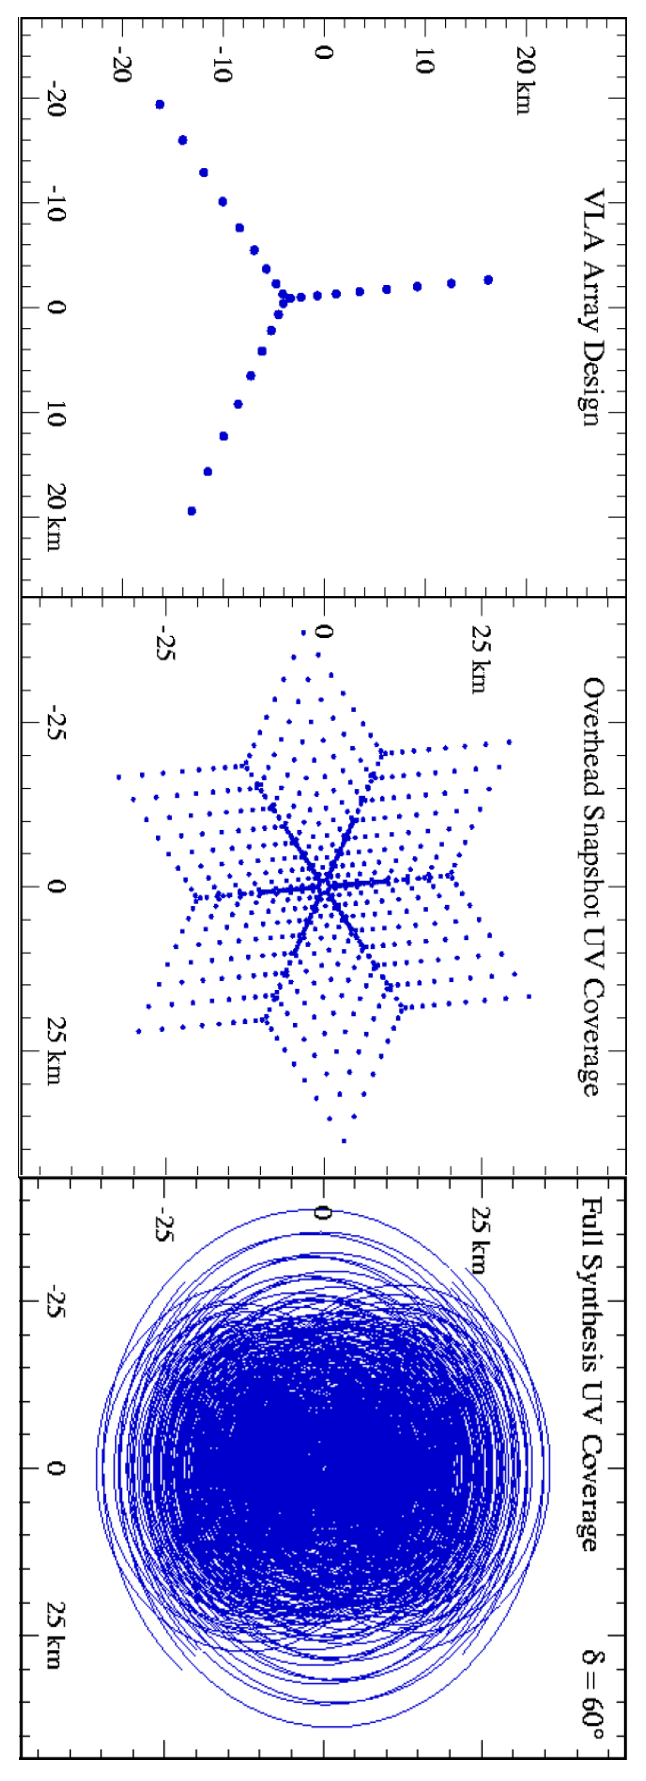
\includegraphics[angle=90,trim=0pt 0pt 0pt 0pt,clip,width=13.5cm, height=5.0cm]{/home/eamon/thesis/figures/uv_coverage.eps}
\caption[VLA antenna layout and two examples of $u-v$ coverage for different track lengths.]{\textit{Left:} The VLA in A-configuration is an example of an `Y' shaped array design. \textit{Middle:} The corresponding overhead snapshot $u-v$ coverage results in `snowflake' pattern. \textit{Right:} The corresponding $u-v$ coverage after a 12 hour track of a source at a declination of 60$^{\circ}$. Note the more intense u-v coverage in the direction of the three straight arms of the VLA for a snapshot track compared to the more uniform coverage over a longer duration track.}
\label{fig2.9}
\end{figure}

\subsection{Imaging (Making a Dirty Map)}\label{subsec:4.2}
For every sky brightness distribution $I(l,m)$ there exists a continuous complex visibility function $V(u,v)$ that is its Fourier Transform. An array of antennas will only ever measure a certain set of values of this visibility function where the measured set is called the sampling function $S(u,v)$. This function is zero where no data have been taken. The actual data provided by the array is known as the sampled visibility function, $S(u,v)V(u,v)$. If we take the inverse Fourrier transform of this function we get what is known as the \textit{dirty image}:

\begin{equation}\label{eq:dirtyim}
I_{\nu}^{D}(l,m)=\int ^{\infty}_{-\infty}\int ^{\infty}_{-\infty}S(u,v)V_{\nu}(u,v)\mathit{e}^{2\pi \mathit{i}(ul+vm)}du\,dv.
\end{equation}
where we have used $I_{\nu}(l,m)$ to denote the modified sky brightness $\mathcal{A}(l,m)I_{\nu}(l,m)$ as the correction for primary beam can be made at the final stage of data processing. Using the convolution theorem, the relationship between the dirty image and the desired intensity distribution $I_{\nu}(u,v)$ is
\begin{equation}\label{eq:dirty_image}
I_{\nu}^{D}(u,v)=I_{\nu}(u,v)*B(l,m)
\end{equation}
where the asterisk implies convolution and
\begin{equation}\label{beam_samp}
B(l,m) = \int ^{\infty}_{-\infty}\int ^{\infty}_{-\infty}S(u,v)\mathit{e}^{2\pi \mathit{i}(ul+vm)}du\,dv
\end{equation}
is the \textit{point spread function} (PSF), or \textit{synthesized beam}, or \textit{dirty beam} (i.e., the inverse Fourrier Transform of the sampling function $S$). Equation \ref{eq:dirty_image} says that the dirty image $I^{D}$ is the true intensity distribution $I$, convolved with the synthesized beam $B$.

In Figure \ref{fig2.10} we graphically summarize what has been said above. The panels in the upper row show the sky plane representations of the true image, the point spread function and the dirty image, while the panels in the lower row show the corresponding $u-v$ plane representations of the true visibility, the sampling function and the sampled visibility. In other words, Equation \ref{eq:2dft} is summarized graphically by the relationship between panels (a) and (d),  Equation \ref{beam_samp} by (b) and (e), and Equations \ref{eq:dirtyim} and \ref{eq:dirty_image} by (c) and (f).

\begin{figure}[hbt!]
\centering 
          \includegraphics[trim=0pt 260pt 0pt 260pt,clip,width=14.0cm]{/home/eamon/thesis/figures/ft_ift.ps}
\caption[The Fourier transform pairs in synthesis imaging.]{The Fourier transform pairs in synthesis imaging. (a) and (d): The true sky brightness and the visibility. (b) and (e): The dirty beam and the sampling function. (c) and (f): The dirty image and the sampled visibility. \textit{Image Credit:} Prof. Dale E. Gary (New Jersey Institute of Technology).}
\label{fig2.10}
\end{figure}

Before the dirty image is computed, a weighting system is often applied to the visibilities to control the PSF. The two most common types of weighting system used are:
\begin{equation}
D_{k}=1,	\ \ \ \ \ \ \ \rm{natural \ weighting}
\end{equation}
\begin{equation}
D_{k}=\frac{1}{N_{s}(k)}, \ \ \ \ \ \rm{uniform \ weighting}
\end{equation}
where $D_{k}$ is the weight to be applied to cell $k$, and ${N_{s}(k)}$ is the number of data samples falling into cell $k$ of characteristic width $s$. Natural weighting treats all points alike and gives the best signal-to-noise ratio for detecting weak sources. However, it produces a beam with a broad low-level plateau which is undesirable when imaging sources with both large and small scale structure. Uniform gridding produces fewer artifacts in the final map, while keeping the full resolution of the array but gives poorer signal-to-noise than natural weighting.

The `direct Fourier transform' method can then be used to solve for the dirty image Equation \ref{eq:dirtyim}. However, if this method is evaluated at every point on a $N\times N$ grid, then the number of multiplications required goes as $N^{4}$. The fast Fourier transform (FFT) algorithm can also be used to solve Equation \ref{eq:dirtyim} but requires interpolating the data onto a regular grid (i.e., a process known as \textit{gridding}). This method is widely used for large data volumes as it requires only a few times $N^{2}\rm{log}_{2}\mathcal{N}$ operations - not $\mathcal{O}(N^4)$, and the total time taken for gridding and FFT is usually a lot less than would take using the direct Fourier transform method.

\subsection{Deconvolution (Making a CLEAN map)}\label{subsec:4.3}
The solution to the inverse Fourier transform given in Equation \ref{eq:2dft}
 is not unique, because the unmeasured points in the $u-v$ plane could have \textit{any} value without violating the data constraints. The `principle solution' is the one in which all missing $u-v$ measurements are set to zero and gives the dirty image discussed in the previous section. The dirty image is usually not a satisfactory representation of the sky as one would expect a more continuous distribution of visibilities than that provided by the array. The goal of the deconvolution process is to find a method that determines more reasonable values for the unmeasured $u-v$ data. A priori information is the key to choosing `reasonable' values. For example, we know that the Stokes parameter $I$ must be positive and that radio sources generally do not have sidelobe patterns.
 
The CLEAN algorithm \citep{hogbom_1974} is the most widely used technique in radio interferometry to deconvolve the true sky intensity from the dirty beam. It assumes that the radio source can be represented by a number of point sources in an otherwise empty field and a simple iterative process is used to find the strengths and positions of these point sources. The final CLEAN image (i.e., the deconvolved image) is the sum of these point sources convolved with a CLEAN beam, which is usually an elliptical Gaussian of the same size and shape as the inner part of the dirty beam. The CLEAN algorithm obeys the following steps:
\begin{enumerate}
\item Find the strength and position of the brightest point in the dirty image. It may also be desirable to search for peaks in specified areas of the image, called CLEAN windows or regions.
\item At this position in the dirty image, subtract the dirty beam multiplied by the peak strength and a damping factor $g$ ($g \le 1$, usually called the loop gain).
\item Record the position and the subtracted flux in a model.
\item Iterate between (1), (2), and (3) until the peak is below some user specified level. The remainder of the dirty image is now  termed the residuals.
\item Convolve the accumulated point source model with an idealized CLEAN beam (usually an elliptical gaussian of the same size and shape as the central lobe of the dirty beam).
\item Add the residuals to the image in (5) to create the final CLEAN image.
\end{enumerate}
A problem with CLEAN is that the final CLEANed image is somewhat dependent upon the various control parameters such as CLEAN boxes, the loop gain and the number of CLEAN subtractions. For example, using too high a gain tends to make extended, weak emission undetectable and noisy. This problem is unavoidable, and input values must be chosen on a case by case basis, depending on the source and data quality.

Another deconvolution algorithm used in radio synthesis imaging, albeit less often, is the Maximum Entropy Method (MEM) which operates by minimizing a smoothness function (`entropy') in an image. To conclude this section, we briefly discuss the practical differences between CLEAN and MEM:
\begin{enumerate}
\item CLEAN is nearly always faster than MEM, unless the image contains more than 1 million pixels.
\item MEM images are nearly always smoother than CLEAN images. This is because for CLEAN, what happens at one pixel is not coupled to what happens to its neighbours, while MEM couples pixels together by minimizing the spread in pixel values.
\item CLEAN sometimes makes extended emission look blotchy and may introduce artificial stripes into the image while MEM copes very poorly with point sources in extended emission. (Multi-scale CLEAN which is discussed in Chaper \ref{chap:3} is now becoming a popular choice in the radio community as an alternative deconvolution algorithm for images containing extended emission.)
% Multiscale CLEAN: http://iopscience.iop.org/1538-3881/136/6/2897/fulltext/
\item For MEM, it is necessary to know the noise level quite well and it also helps to know the total flux density of the image. Knowledge of these are not required for CLEAN.
\end{enumerate}

